\chapter{تخصیص منابع در شبکه‌های دسترسی رادیویی باز}
\section{مقدمه}
در اینحا هدف ما، فرمول بندی برش RAN برای معماری O-RAN است. این مطالعه، تکنیکی را برای ایجاد خطوط کلی برش شبکه ایزوله در معماری O-RAN برای ارائه QoS خاص برای eMBB، URLLC و mMTC ارائه می‌کند. علاوه بر منابع باند پایه، تعداد VNF ها نیز برای کاهش تأخیر به ویژه برای خدمات URLLC، در نظر گرفته می شود.
در این بخش هدف تخصیص منابع در ساختار شبکه های دسترسی رادیویی باز با استفاده از برش شبکه برای سرویسهای مختلف با کیفیت سرویس متفاوت باتوجه به شکل \ref{fig:c11} می باشد. 
خلاصه‌ی مهم‌ترین نوآوری‌های این بخش بدین صورت است:
\begin{itemize}
	\item 
	در اینجا یک مدل برش شبکه را برای سه سرویس مختلف معرفی شده در \lr{5G}، یعنی eMBB، mMTC و URLLC به تصویر می‌کشد. در معماری O-RAN، مشکل تخصیص منابع رادیویی و فعال سازی VNF بررسی می شود.
	ما بر اساس انواع مختلف خدمات با اولویت ها و QoS مختلف، یک مسئله برای تخصیص منابع باند پایه برای به حداکثر رساندن توان عملیاتی وزنی O-RAN فرموله می کنیم.
	\item 
	ما دراینجا تأخیر پردازش و منابع VNF مورد نیاز برای برش را در مقایسه با سایر مقالات در نظر گرفته‌ایم. بنابراین، ما بر به دست آوردن تعداد بهینه VNF در هر لایه از معماری O-RAN تمرکز می نماییم.
	همچنین سرویسهای مختلف با QoS مختلف شامل تاخیر، توان و نرخ را بررسی نموده‌ایم و با توجه به تعداد VNFهای فعال شده و نرخ هر کابر، تاخیر پردازشی انتها به انتها را بدست می‌اوریم.
	
	با فرض ظرفیت محدود فرانتهال، توان و ظرفیت واقعی هر O-RU را محاسبه می کنیم. بسته به نوع سرویس، تداخل O-RUهای همسایه را مدل کرده و نرخ را تعیین می‌نماییم. در مدل سیستم در نظر گرفته شده، انتقال بسته کوتاه URLLC و mMTC را به حساب می‌آوریم که نمی‌توان با قضیه ظرفیت شانون مدل‌سازی کرد.
\item 	
مسئله‌ی مورد بررسی، یک مسئله‌ی غیرخطی همراه با  ترکیب اعداد صحیح و پیوسته است که برای حل آن از یک الگوریتم دو مرحله‌ای تکراری استفاده می‌نماییم که در مرحله‌ی اول، تعداد VNFهای فعال، تخصیص توان و PRB بدست می‌آید و در مرحله‌ی دوم ارتباط کاربران با o-RU ها بدست می‌آید.
\item 
ما مسئله‌ی اصلی را در مرحله‌ی اول برای یافتن یک کران بالا و پایین برای تعداد VNF های فعال شده مجدداً فرموله و ساده می کنیم و از تابع لاگرانژی و شرایط KKT برای یافتن توان بهینه و تخصیص PRB استفاده می کنیم.
برای مرحله دوم، مسئله‌ی ارتباط O-RU را می توان به یک مسئله‌ی کوله پشتی چندگانه تبدیل کرد و با الگوریتم حریصانه حل کرد.
\item 
در نهایت، بحث در مورد انتخاب نقطه اولیه و منطقه امکان پذیر برای نتایج عددی ارائه شده است. همچنین، ما یک الگوریتم سریع را معرفی می‌کنیم که پیچیدگی کمتری نسبت به روش ما برای تحقق بخشیدن به منطقه امکان‌پذیر برای مسئله‌ی ما دارد. 
\end{itemize} 

\begin{figure}
  \centering
  \captionsetup{justification=centering}
    \includegraphics[scale = 0.4]{./img/finalDraw1.pdf}
    %\includegraphics[width=9.cm,height=6.2cm]{finalDraw1.pdf}
    %\includegraphics[width=\textwidth]{finalDraw.pdf}
  \caption{برش شبکه در سیستم O-RAN}
  \label{fig:c11}
\end{figure}
در ادامه‌ی این فصل، ابتدا مدل سیستم و فرمولاسیون مسئله را بیان می‌نماییم. سپس الگوریتم مورد نظر را ارائه داده و در نهایت     نتایج عددی رو بیان می کنیم.

\section{مدل سیستم و فرمولاسیون مسئله}\label{systemmodel}
در این بخش، سیستم فروسو \LTRfootnote{Downlink} را در معماری O-RAN با استفاده از برش RAN همانطور که در شکل \ref{fig:c11} نشان داده شده است، توصیف می کنیم.
ابتدا مدل سیستم را ارائه می کنیم. سپس، نرخ‌های داده قابل دستیابی، توان O-RU و ظرفیت فرانتهال برای لینک فروسو سیستم O-RAN را به دست می‌آوریم. پس از آن، میانگین تاخیر و توان VNF ها را مورد بحث قرار می دهیم.
در نهایت مسئله‌ی اصلی بیان می شود.
\subsection{مدل سیستم}
فرض کنید، سه نوع سرویس شامل eMBB، URLLC و mMTC وجود دارد که از برنامه های مختلف پشتیبانی می کنند.
بر این اساس، برش‌های $S_1$ برای نوع سرویس اول (eMBB)، برش‌های $S_2$ برای نوع سرویس دوم (URLLC) و برش‌های $S_3$ برای نوع سرویس سوم (mMTC) وجود دارد.

بنابراین،  $S$ برش‌ از پیش تخصیص داده شده وجود دارد که به این $S$ سرویس، خدمات ارائه می‌کنند ($S = S_1 + S_2 + S_3$).
بنابراین، هر درخواست سرویس $s\in \{1,\ldots,S\}$ توسط بخش مربوطه ارائه می‌شود.
بنابراین  $\{1,2,...,S_1\}$ 
مجموعه ای از نمونه‌های سرویس 
eMBB
می‌باشد. همچنین
 $\{1,2,...,S_2\}$ 
  مجموعه‌ای از نمونه‌های سرویس  URLLC
  است. 
   و $\{1 داریم. ,2,...,S_3\}$ مجموعه نمونه های سرویس mMTC می‌باشد.
   
   هر سرویس $s_j\in \{1,2,...,S_j\} $ شامل درخواست‌های $U_{s_j}$ از UE‌های تک آنتنی است که به سطح خاصی از QoS نیاز دارند.
   همچنین $j \in \{1,2,3\}$ نوع سرویس را نشان می‌دهد.
   درخواست های کاربردی مختلفی وجود دارد که در یکی از این دسته خدمات قرار می گیرند. هر درخواست برنامه به QoS خاصی نیاز دارد. بر اساس درخواست و QoS، UE ممکن است پذیرفته شده و به منابع اختصاص یابد.
   
   
   
   
   
   
   